\documentclass[a4paper,10pt]{article}

\usepackage[spanish]{babel}
\usepackage[utf8]{inputenx}
\usepackage{booktabs}
\usepackage{multirow}
\usepackage{amssymb}
\usepackage{graphicx}
\usepackage{listings}
\usepackage{verbatim}
\newcommand{\here}{\checkmark}

\newenvironment{code}{\footnotesize\verbatim}{\endverbatim\normalsize}
\DeclareUnicodeCharacter{03BB}{$\lambda$}
\DeclareUnicodeCharacter{2192}{$\rightarrow$}

\title{Implementación de Lenguajes: Attribute Grammars}
\author{Alejandro Gadea \and Emmanuel Gunther}

\begin{document}
\maketitle
\lstset{ language=Haskell
       , literate={λ}{{$\lambda$}}1
	   }

\section{Sintaxis y semántica de Lenguajes}

\subsection{El problema RepMin}

El problema ``Rep Min'' es un ejemplo famoso del poder de la evaluación Lazy e inspira la construcción
de la manera de definir semántica que explotan las Attribute Grammars.

Consideremos el tipo de dato de los árboles binarios, con números enteros en las hojas. El problema
consiste en reemplazar cada valor de las hojas del árbol por el valor mínimo:

\begin{center}
 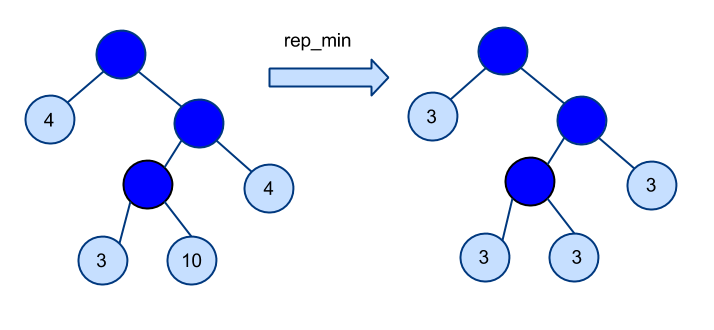
\includegraphics[height=4cm]{./repmin.png}
\end{center}

Podríamos definir un tipo de dato en Haskell para representar un árbol binario
de la siguiente manera:

\begin{lstlisting}
 data Tree =   Leaf Int 
	     | Bin (Tree,Tree)
\end{lstlisting}

Un árbol puede construirse a partir de un entero (una hoja) o a partir de otros
dos subárboles. Es decir, podemos construir un elemento de $Tree$ a partir
de un elemento de la unión disjunta $Int \sqcup (Tree\,\times\,Tree)$.
A esta unión disjunta la podemos definir en Haskell para cualquier tipo $a$:

\begin{lstlisting}
 type FTree a = Either Int (a,a)
\end{lstlisting}

\noindent y entonces podemos obtener cualquier elemento de $\mathbf{Tree}$ a partir de algún elemento de
$\mathbf{FTree\,Tree}$.

Al tipo de esta función que consiste en obtener un elemento de tipo $a$ a partir de uno de tipo
$\mathbf{FTree}\,a$ lo definimos explícitamente:

\begin{lstlisting}
 type FTreeAlgebra a = FTree a -> a
\end{lstlisting}



Si queremos definir entonces una semántica para los árboles binarios en un conjunto
semántico $B$ podemos definir una $\mathbf{FTreeAlgebra}\;B$. Para ello tenemos que dar
una regla para el caso en que partimos de un entero y otra regla para el caso en el que 
partimos de un par en $B\;\times\;B$.

La representación sintáctica de los árboles binarios con el tipo $Tree$ podría verse como una
semántica trivial y la podemos definir de la siguiente manera:

\begin{lstlisting}
  init_algebra :: FTreeAlgebra Tree
  init_algebra = either Leaf Bin
\end{lstlisting}

Si pensamos en términos de categorías, podemos ver a $FTree$ como un funtor que transforma
un objeto $A$ en un objeto $Int \sqcup (A\,x\,A)$ y entonces una $FTree-algebra$ será un morfismo
$\alpha\,:\,FTree\;A\;\rightarrow\;A$. Si $\alpha$ es la FTree-álgebra inicial entonces para cualquier otra
FTree-álgebra $\beta\,:\,FTree\;B\;\rightarrow\;B$ debe existir un único morfismo entre $\alpha$ y $\beta$, 
es decir, una única $f$ tal que el siguiente diagrama conmuta:

\begin{center}
 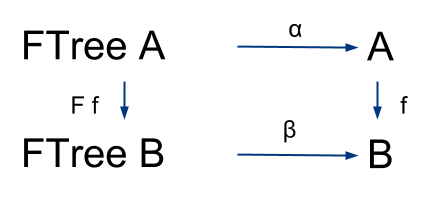
\includegraphics[height=3cm]{./Falgebras.png}
\end{center}

Si queremos entonces dar semántica a los árboles binarios debemos encontrar el único morfismo
entre $init\_algebra$ (el FTree-álgebra inicial) y otra FTree-álgebra. A este morfismo
se lo llama \textbf{catamorfismo}:

\begin{lstlisting}
  cataTree :: FTreeAlgebra b -> Tree -> b
  cataTree beta (Leaf i)    = beta (Left i)
  cataTree beta (Bin (t1,t2)) = beta (Right (cataTree beta t1,
					     cataTree beta t2))
\end{lstlisting}


Volviendo al problema que queremos resolver, a partir de un árbol queremos obtener
otro en el cual los valores de las hojas están reemplazados por el mínimo.

Una primera solución consiste en primero obtener el mínimo del árbol y luego reemplazar
por ese valor encontrado todas los valores de las hojas. Esto implica realizar dos 
recorridas al árbol inicial.

Para obtener el mínimo definimos una FTree-álgebra y definimos una función
que dado un entero $n$ construye la FTree-álgebra para reemplazar
los valores de las hojas por $n$:

\begin{lstlisting}
  min_alg :: FTreeAlgebra Int
  min_alg = either id (uncurry min)

  rep_min_alg :: Int -> FTreeAlgebra Tree
  rep_min_alg n = either (const $ Leaf n) Bin
\end{lstlisting}

Encontramos el resultado entonces llamando a la función $cataTree$
dos veces:

\begin{lstlisting}
  replace_min :: Tree -> Tree
  replace_min t = let n = cataTree min_alg t in
		      cataTree (rep_min_alg n) t
\end{lstlisting}



% de los árboles binarias con el tipo $Tree$ constituyen el álgebra inicial, que consiste en
% aplicar la función $Leaf$ si el elemento es un entero, y la función $Bin$ si 



\subsection{Repmin con Attribute Grammars}

\section{El cálculo Lambda}

En la sección pasada vimos como podemos definirnos una función de manera general,
que llamábamos catamorfismo, y como esta definición nos induce la introducción
de una sintaxis especial con la idea de que solo haga falta implementar lo relativo
al problema. 

A continuación vamos a implementar un inferidor de tipos para el cálculo lambda 
simplemente tipado, así también como su parser y pretty printing.

\subsection{Sintaxis: Parser y Pretty Printing}

\subsubsection{Sintaxis}

$Var$ $::=$ Conjunto numerable. En general serán $a$, $b$, $c$, $x$, $y$, $z$, etc.


\begin{lstlisting}
Term ::= Var
       | λ Var . Term
       | Term Term
\end{lstlisting}


\subsubsection{Parser}

La implementación de un parser para la sintaxis del calculo lambda es mas bien
simple y directa, aun incluso agregando la restricción de que solo permitimos parsear
términos cerrados, es decir términos en los cuales no aparecen variables libres.
Sin embargo, supongamos tenemos el siguiente termino a parsear,\\

$\lambda a . s$\\

claramente ``s'' es libre, pero no estaría mal suponer que en realidad ese termino
bien podría haber sido\\

$\lambda a . a$\\

es decir, se cometió un error al escribir el termino. Por lo tanto, un parser
algo mas interesante podría ser uno tal que detecte este tipo de errores, los
corrija e informe sobre tal decisión.\\

Ahora bien, para la implementación del parser utilizamos la librería "uu-parsinglib"
la cual provee exactamente una corrección de errores. Por ejemplo, siendo "pa"
el parser de la letra "a", al intentar parsear "b" obtenemos "a" donde lo que
sucedió fue el reemplazo de "b" por "a":\\

\begin{code}
 >>> run pa  "b"
     Result: "a"
     Correcting steps: 
       Deleted   'b' at position LineColPos 0 0 0 expecting 'a'
       Inserted  'a' at position LineColPos 0 1 1 expecting 'a'
\end{code}

Algo a destacar es que la corrección de errores que pretendemos para nuestro
parser de términos es casi gratuita. En un resumen preliminar, para parsear el
cuerpo de una abstracción solamente tenemos que tener una lista de las variables
introducidas hasta ese momento y generar parser's para cada nombre de variable
en esa lista.\\

Antes de presentar los parser relativos a cada construcción de la gramática,
definamos algunos parsers generales que nos van a ser de utilidad.

\begin{lstlisting}
parseTermSym :: Parser String -> [String] -> Parser String
\end{lstlisting}
Generamos un parser a partir de un parser por default y una lista de strings.

\begin{lstlisting}
parseXSym :: Parser String
\end{lstlisting} con X $\in$ {Lam,Dot,App}\\

Parsers para los símbolos $\lambda$, $.$ y $@$. Donde además podemos parsear 
``\textbackslash \textbackslash'' en lugar de $\lambda$ y $->$ o $\rightarrow$
en lugar de ``$.$'' .

\begin{lstlisting}
parseVar :: Parser Var
\end{lstlisting} Parser de variables.\\

Ahora sí, dada la lista de variables a parsear, digamos $vars$, parsear un
identificador de variable será generar parsers para cada variable de la lista
y fallar parser default:

\begin{lstlisting}
parseId :: [Var] -> Parser Term
parseId vars = Id <$> parseTermSym pFail vars
\end{lstlisting}

Lo interesante a destacar es que en la generación de parsers para las variables,
esta contenida la acción de corregir una ocurrencia de variable libre.\\

Para el caso de la abstracción, dejando de lado el parseo de los símbolos respectivos,
vamos a parsear una variable y se podría decir que la necesitamos para dos cosas;
(1) el constructor de la abstracción, (2) la lista de variables posibles a parsear.
Esto genera un problema, ya que al parsear la variable esta queda encapsulada 
dentro de la computación "Parser Var", por (2) podemos pensar que el parser encargado
de parsear el cuerpo de la abstracción tiene el siguiente tipo Var -> Parser Term,
ya que toma la variable la añade a la lista de variables y parsea el termino.
Si ahora prestamos atención necesitamos una función que convine, parsear la variable con
parsear un termino agregando esa variable, es decir una función con tipo:

\begin{lstlisting}
Parser Var -> (Var -> Parser Term) -> Parser Term
\end{lstlisting}

pero este es justamente el tipo del bind ($>>=$), $m \ a \rightarrow (a \rightarrow m \ b) \rightarrow m \ b$. Esto
nos obliga a usar mónadas entonces para lo cual necesitamos la función addLength.
No estamos seguros si existe una manera de resolver esto sin usar mónadas, con el
fin de evitar el uso de addLength. La definición final entonces queda,

\begin{lstlisting}
parseAbs :: [Var] -> Parser Term
parseAbs vars = 
       addLength 1 $
       join $ uncurry (<$>) 
           <$> 
       (Abs &&& parseTerm . (:vars))
       	   <$ 
       parseLamSym <*> parseVar <* parseDotSym
\end{lstlisting}

Concluyendo, para el caso de la aplicación será parsear identificadores de variable
o abstracciones separadas por ``$@$'', para esto nos definimos un parser particular
para estos parsers,

\begin{lstlisting}
parseTerm' :: [Var] -> Parser Term
parseTerm' vars =  parseId vars
               <|> parseAbs vars
               <|> pParens (parseTerm vars)\\

parseApp :: [Var] -> Parser Term
parseApp vars = (App <$ parseAppSym) `pChainl` (parseTerm' vars)
\end{lstlisting}

luego, parsear un termino será simplemente el parser definido para la applicación,\\

\begin{lstlisting}
parseTerm :: [Var] -> Parser Term
parseTerm vars = parseApp vars
\end{lstlisting}

En conclusión, tenemos un parser para la gramática anterior que además corrige 
algunos errores, como el mencionado al comienzo. Algo importante a mencionar es
que la corrección de errores puede tener algún que otro comportamiento no deseado
como consecuencia de una implementación "simplista" en términos del uso del 
poder de corrección de la librería. Un ejemplo de esto podría ser,

\begin{verbatim}
*Parser> parserTerm "\\a -> b@a"
(λ a → a
, [-- Deleted   'b' at position LineColPos 0 6 6 expecting Whitespace
  ,-- Deleted   '@' at position LineColPos 0 7 7 expecting "a"
  ]
)
\end{verbatim}

donde muy probablemente la corrección deseada hubiera sido simplemente reemplazar
b por a, y generar el termino $\lambda$ a $\rightarrow$ a@a.


\subsection{Inferidor de tipos}
 
\end{document}
